% mycsrf 'for beeing included' snippet template
%
% (c) Karsten Reincke, Frankfurt a.M. 2012, ff.
%
% This text is licensed under the Creative Commons Attribution 3.0 Germany
% License (http://creativecommons.org/licenses/by/3.0/de/): Feel free to share
% (to copy, distribute and transmit) or to remix (to adapt) it, if you respect
% how you must attribute the work in the manner specified by the author(s):
% \newline
% In an internet based reuse please link the reused parts to mycsrf.fodina.de
% and mention the original author Karsten Reincke in a suitable manner. In a
% paper-like reuse please insert a short hint to mycsrf.fodina.de and to the
% original author, Karsten Reincke, into your preface. For normal quotations
% please use the scientific standard to cite
%

\section{w01: Easy\-ABC \ra\ abc2mtex \ra\ \LaTeX+Musix\TeX}\label{w01}

Im Ordner \texttt{[\ldots]/musicology.de/chain-evaluation/} in den Quellen zu
diesem Dokument\footcite[vgl.][\nopage wp]{Reincke2019a} haben wir
den weg-spezifischen Subordner \texttt{w01-easyabc-abc2mtex} generiert.
Er enthält zunächst einen Subordner \texttt{tools}, in dem das Frontend
\acc{EasyABC} und die Quellen des Konverters \acc{abc2mtex} als Paket abgelegt
sind. Entpackt man das Paket \texttt{abc2mtex1.6.1.tar.gz}, kann man --
weg-spezifischen Subordner aus -- mittels \texttt{tools/abc2mtex} den Konverter
aufrufen. In diesem Wegeordner liegt unter dem Namen
\texttt{easyabc-cadenca3.abc} auch die ABC-Version unser Kadenz III, wie wir sie
in und mit \acc{EasyABC} generiert haben.

Damit sollte man dem Konverter \acc{abc2mtex} nun an der Kommandozeile die
\acc{ABC}-Datei als Parameter übergeben können und die konvertierte
\acc{Music\TeX}-Datei zurückerhalten:

\begin{quote}\texttt{tools/abc2mtex easyabc-cadenca3.abc}\end{quote}

Leider bricht das Programm mit einer Fehlermeldung ab:

\begin{quote}\texttt{error in input file easyabc-cadenca3.abc: line no. 10 - V
field not allowed in tune body }\end{quote}

Das ist 'leicht' erklärbar: Das ABC-Format war ursprünglich ein
Notationsverfahren für einstimmige 'Lieder'.\footnote{\ra\ S. \pageref{ABCMethod}}
Es ist erst später zu einem 'patitur-fähigen' Format erweitert worden. Der
Konverter \acc{abc2mtex} versteht nun offensichtlich nur das alte Format.
 
Daraus folgt leider, dass wir offensichtlich (noch) kein Verfahren haben, um 
Notentexte im \acc{Music\TeX}-Format über ein Frontend zu erfassen, und zwar auch
dann nicht, wenn das Zielformat erst über einen Konverter erzeugt werden darf.

\section{w02: Easy\-ABC \ra\ abc2ly  \ra\ Frescobaldi \ra\ \ldots}\label{w02}

Außerdem haben wir in dem Ordner \texttt{[\ldots]/musicology/chain-evaluation/}
den weg-spezifischen Subordner \texttt{w02-easyabc-abc2ly} erzeugt. Auch hier
haben wir ABC-Version unser Kadenz III abgelegt, wie wir sie in und mit
\acc{EasyABC} generiert hatten:

\begin{center}
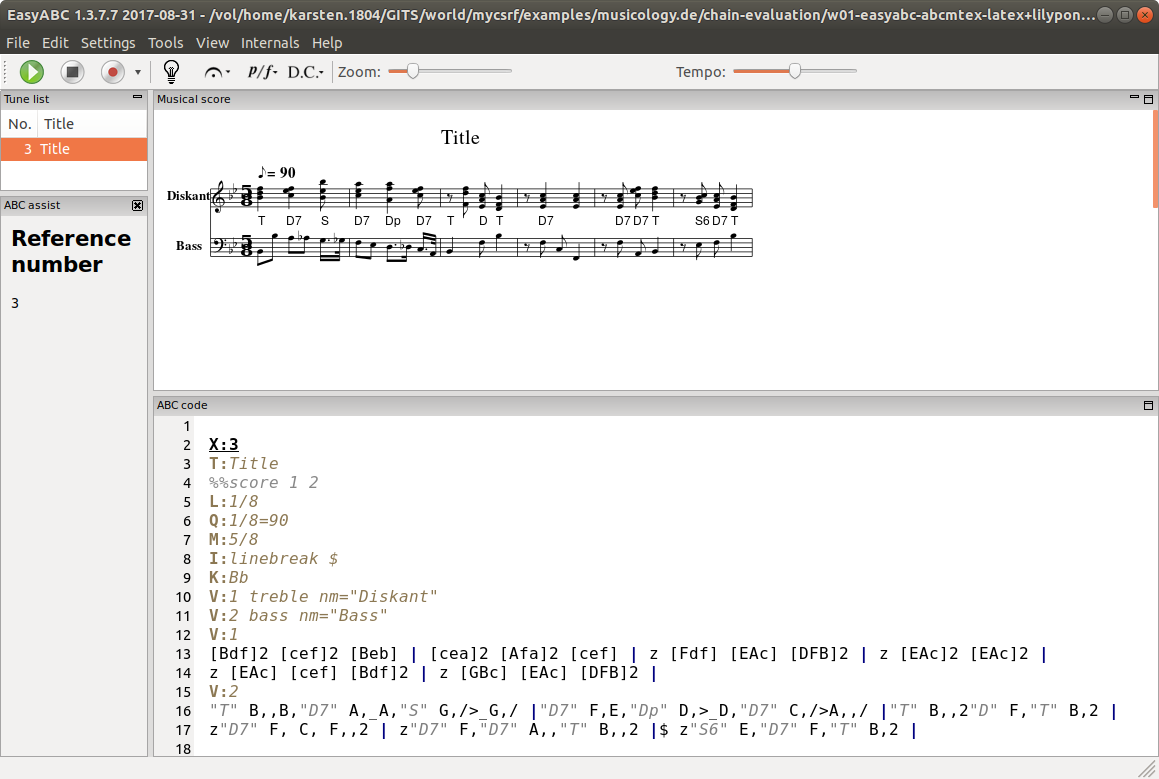
\includegraphics[width=0.9\textwidth]{frontends/easyabc/easyabc-cadenca3.png}
\end{center}

Mit dem folgenden Befehl kann man diese \acc{ABC}-Outputdatei in eine
\acc{LilyPond}-Datei konvertieren:

\begin{quote}\texttt{abc2ly -o easyabc-cadenca3.ly easyabc-cadenca3.abc}\end{quote}

Betrachtet man das Ergebnis in Frescobaldi, sieht man, dass die Konvertierung
nur sehr bedingt funktioniert hat:

\begin{center}
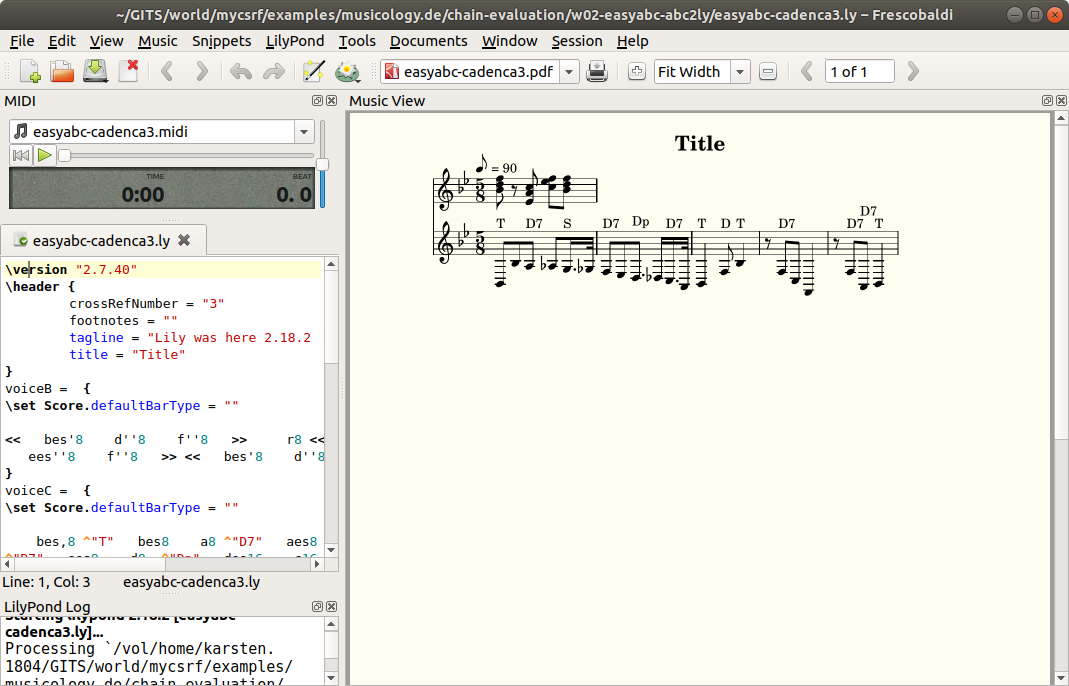
\includegraphics[width=0.9\textwidth]{frontends/easyabc/easyabc-cadenca3-in-frescobaldi.png}
\end{center}

Daran ändert sich auch nichts, wenn man aus der \acc{EasyABC} die 'Texte'
entfernt und nur die Noten erfasst. Wir dürfen also sagen, dass man
\acc{EasyAbc} auch mit Konverter nicht wirklich als Frontend für \acc{LilyPond}
verwenden kann.

\section{w03: Muse\-Score \ra\ musicxml2ly \ra\ Frescobaldi \ra\ \ldots}\label{w03}

Schließlich haben wir in dem Ordner
\texttt{[\ldots]/musicology/chain-evaluation/} den weg-spezifischen Subordner
\texttt{w03-musescore-musicxml2ly} erzeugt und darin die Kandenz-III als
\acc{MuseScore}-Datei (\texttt{cadenca3.mscz}) und den korrespondierenden
MusicXML-Output (\texttt{cadenca3.xml})abgelegt:

\begin{center}
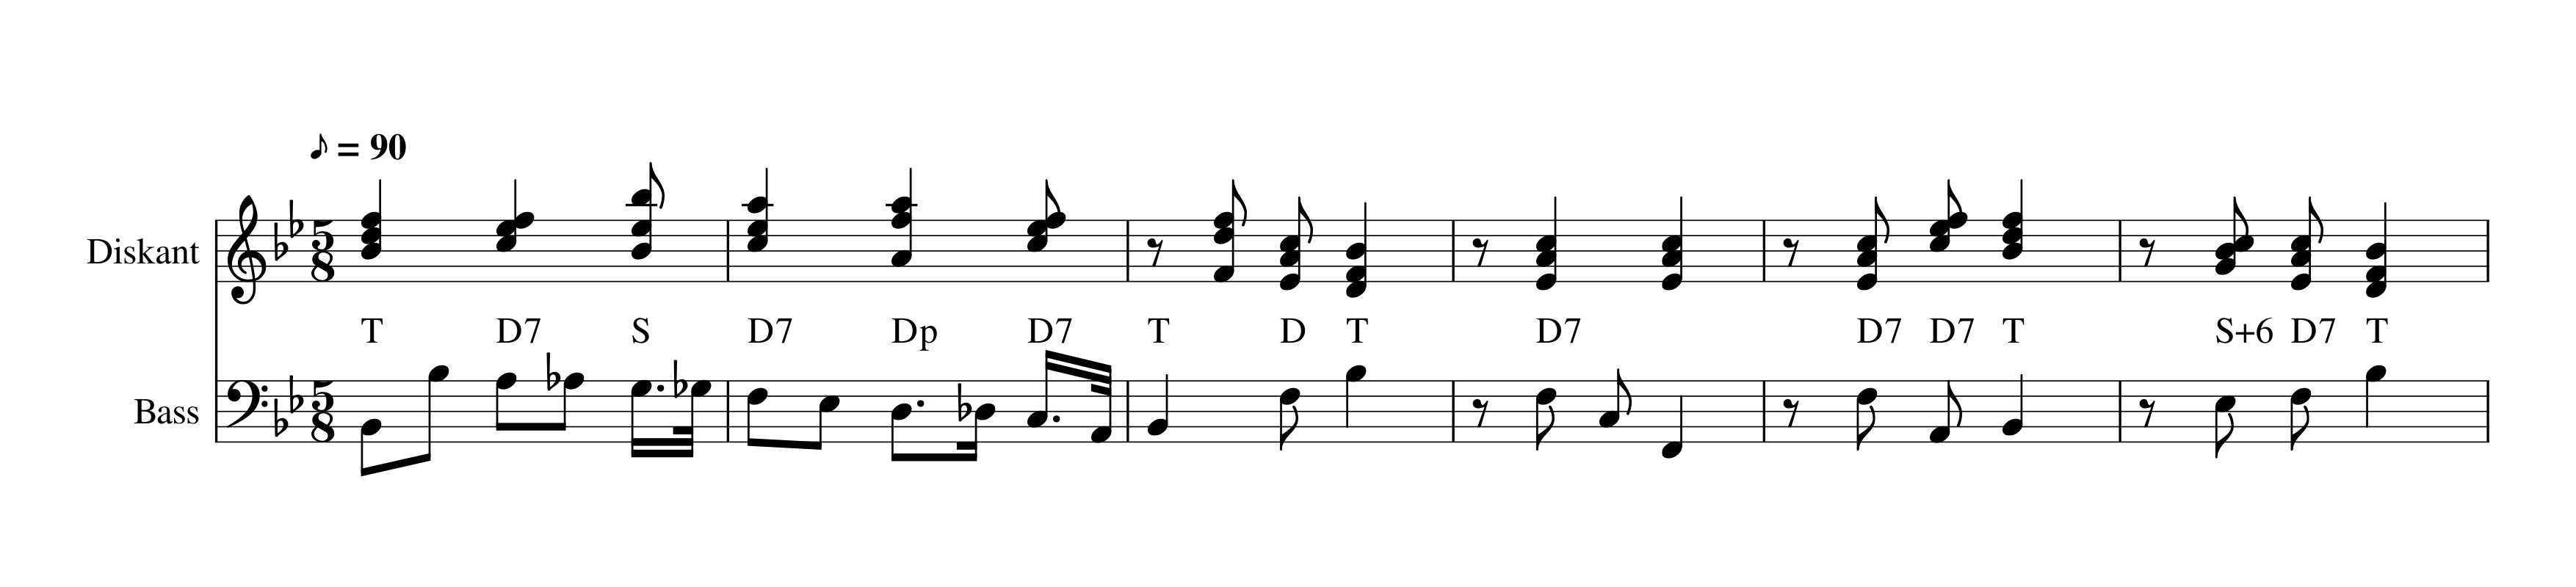
\includegraphics[width=0.9\textwidth]{frontends/musescore/cadenca3-musescore-300dpi.png}
\end{center}

Damit sollte sich auch die XML-Datei in eine \acc{LilyPond}-Datei konvertieren lassen:

\begin{quote}\texttt{musicxml2ly -o cadenca3.ly cadenca3.xml}\end{quote}

Technisch läuft die Konvertierung problemlos durch. Das Ergebnis sieht in
\acc{Frescobaldi} nicht so schlecht aus:


\begin{center}
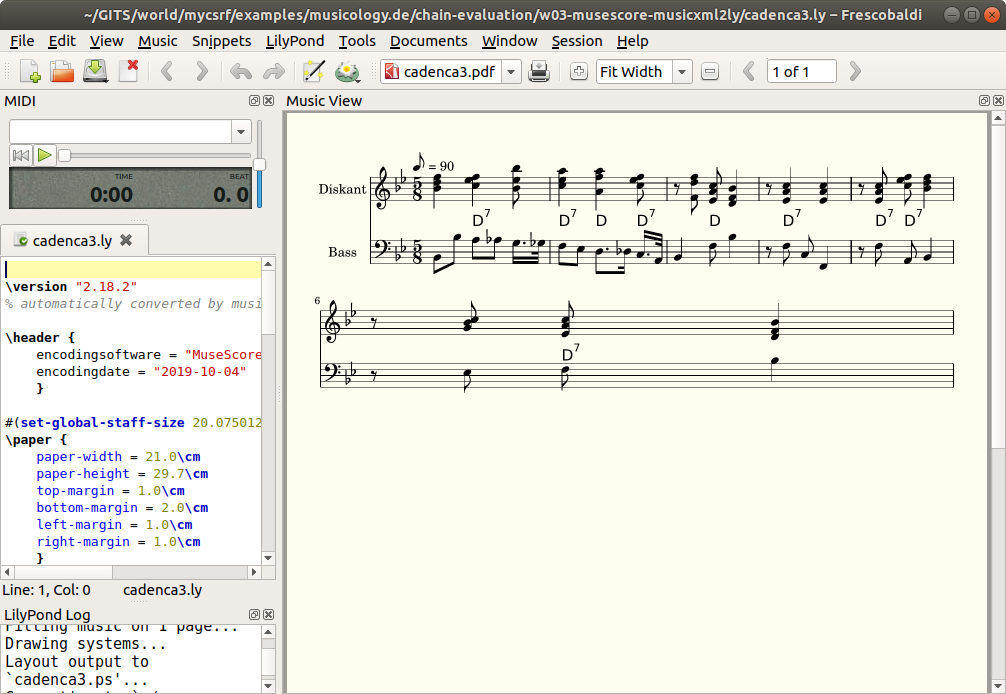
\includegraphics[width=0.9\textwidth]{frontends/musescore/musescore-cadenca3-in-frescobaldi.png}
\end{center}

Einzig sind einige Harmoniesymbole unter den Tisch gefallen, die eh durch die
äquivalenten Ausdrücke über unser Zusatzbibliothek \acc{harmonyli} ersetzt
werden sollen.

Damit dürfen wir sagen, dass man \acc{LilyPond} auch mit einem echten
graphischen Frontend verwenden kann, nämlich mit \acc{MuseScore}, sofern man
auch den von \acc{LilyPond} gepflegten Konverter \acc{musicxml2ly}
verwendet. Dass das Frontend \acc{MuseScore} von sich aus keine adäquaten
Harmonieanalysesymbole mitbringt, ist kein Nachteil: man lässt sie ja eh
weg, um später über die semi-graphische Editoren \acc{Frescobaldi} oder
\acc{Elysium} die Syntagmen nachzutragen, die die Bibliothek \acc{harmonyli.ly}
in die Gesatltung einbringt.


\section{Vergleich in Tabellenform}

\begin{footnotesize}

\begin{tabular}{|c||c|c|c|c|c||c||}

% was soll am Anfang oben scheinen:
\hline
  \multirow{2}{*}{\rotatebox{90}{Weg\ }} & \multicolumn{2}{c}{VON} & \multicolumn{1}{|c}{ÜBER} & 
  \multicolumn{2}{|c||}{NACH} & WERTUNG \\
\cline{2-7}
 & Frontend & $\bigstar$ & Konvertierung & \LaTeX\ + & $\bigstar$ &  \\
\hline
\hline
01 & EasyABC & 4 & \ra\ abc2mtex \ra\ & Musix\TeX\ & 4 &  \texttt{--} \\
\hline
02 &  EasyABC & 5 & \ra abc2ly \ra\ Frescobaldi \ra\ & LilyPond & 5 & \texttt{-} \\
\hline
03 &  MuseScore & 5 & \ra musicxml2ly \ra\ Frescobaldi \ra\ & LilyPond & 5 & \texttt{++} \\
\hline
04 &  Frescobaldi & 5 & \ra\ & LilyPond & 5 & \texttt{++}  \\
\hline
\hline
\end{tabular}

\end{footnotesize}
